%%%%%%%%%%%%%%%%%%%%%%%%%%%%%%%%%%%%%%%%%%%%%%%%%%%%%%%%%%%%%%%%%%%%%%
%%                     Entity
%%%%%%%%%%%%%%%%%%%%%%%%%%%%%%%%%%%%%%%%%%%%%%%%%%%%%%%%%%%%%%%%%%%%%%
%\color{blue}

\subsubsection{Glyph: \glyph{Entity}}
\label{sec:entity}

\SBGNERLone defines only one glyph for all entities, whether physical entity, such as protein, a nucleic acid, metabolite or functional entity such as a gene. Indeed the exact nature of entities does not impact the rules of interactions within a diagram. The nature of a particular entity may then be clarified using its label and decorations, as will become clear below. 

\begin{glyphDescription}

\glyphSboTerm SBO:0000245 ! entity 

\glyphContainer An \glyph{entity} is represented by a rectangular container with rounded corners, as illustrated in \fig{entity}.

\glyphLabel An \glyph{entity} is identified by a label placed in an unbordered box containing a string of characters.  The characters can be distributed on several lines to improve readability, although this is not mandatory.  The label box must be attached to the center of the container. The label may spill outside of the container. 

\glyphAux An \glyph{entity} might carry state variables that can add information about its state (\sect{stateVariable}).  A state variable is represented by a ``stadium'', that is a rectangle capped with two hemi-circles, with the long axis of this stadium placed on the border of the \glyph{entity}'s container, as illustrated in \fig{entity}.  The label of the state variable (which can precise the type of characteristic represented by the state variable, residue type, residue number etc.) is written within the state variable's container. Particular \glyph{state variables} are the existence (\sect{existence}) and the location (\sect{location}).

An \glyph{entity} can carry one or several \glyph{units of information} (\sect{unitInformation}).  Particular \glyph{units of information} are available for describing the material type (\sect{material-types-cv}) and the conceptual type (\sect{conceptual-types-cv}) of a macromolecule.  The center of the bounding box of a \glyph{unit of information} is located on the mid-line of the border of the macromolecule.
% 
% An \glyph{entity} can carry one of several \glyph{domains}. \glyph{Domains} are represented by labelled subsections of the \glyph{entity}. The leftward section represents the whole entity. 

\end{glyphDescription}

\begin{figure}[H]
  \centering
  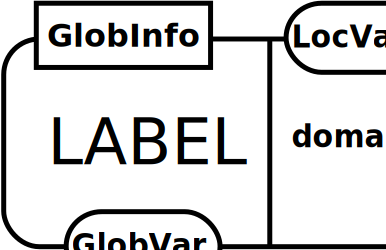
\includegraphics[scale = 0.3]{images/entity}
  \caption{The \ER glyph for \glyph{entity}, showing a unit of information (\sect{unitInformation}), and two state variables (\sect{stateVariable}). The state variables can be carried by the same \glyph{entity}, or two \glyph{entities} with the same name, representing the same concept.}
  \label{fig:entity}
\end{figure}

\begin{figure}[H]
  \centering
  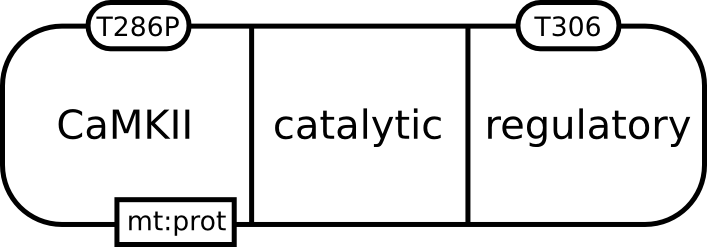
\includegraphics[scale = 0.5]{examples/ex-entity}
  \caption{Example of an \glyph{entity} named CaMKII, that carries two \glyph{state variables} representing the phosphorylated residu threonine 286, and the residu threonine 306, a \glyph{unit of information} precising its material status (protein), and two \glyph{units of information} used to anchor specific \glyph{interactions}.}
  \label{fig:ex-entity}
\end{figure}

%\normalcolor
